\section{Convolutional Neural Networks}
\subsection*{Convolution Definition}Let $f,h$ be functions, their convolution is defined as:\\
\begin{inparaitem}[$\color{mygreen} \triangleright$]
\item Continuous: $(f * h)(u) := \int_{-\infty}^{\infty}f(t)\cdot h(u-t)dt$.\\
\item Discrete: $(f * h)(u) := \sum_{-\infty}^{\infty}f[t] \cdot h[u-t]$\\
\end{inparaitem}
 $h$ is often called the \textit{kernel} convolving with $f$.
\subsection*{Properties}
\begin{inparaitem}[$\color{mygreen} \triangleright$]
\item Commutativity: $(f * h)(u) = (h * f)(u)$\\
\item Shift equivariance: Let $f_{\Delta}(t) = f(t + \Delta)$. Then it holds that $f_{\Delta} * h = (f * h)_{\Delta}$\\
\item Any linear shift-equivariant transformation $T$ can be written as a convolution with a suitable $h$.
\end{inparaitem}
\subsection*{Applications}
\begin{inparaitem}[$\color{mygreen} \triangleright$]
\item Reducing the effect of symmetrically-distributed noise on a signal. Let $x[t] = s[t] + \epsilon[t]$ be a noisy observation of the signal $s$. Convolving $x[t]$ can help to cancel out / reduce the noise $\epsilon$.
\end{inparaitem}
\subsection*{Deconvolution and Cross-correlation}
\term{Deconvolution}: Given $g = f * h$, the goal is to recover $f$. This is only possible under additional assumptions.\\
\term{Cross-correlation}: $(h \star f)[u] := \sum_{-\infty}^{\infty}h[t]\cdot f[u+t]$. Closely related to convolution: $(h \star f) = (\bar{h} * f)$ where $\bar{h}[t] := h[-t]$
\subsection*{Convolutional Neural Network}
%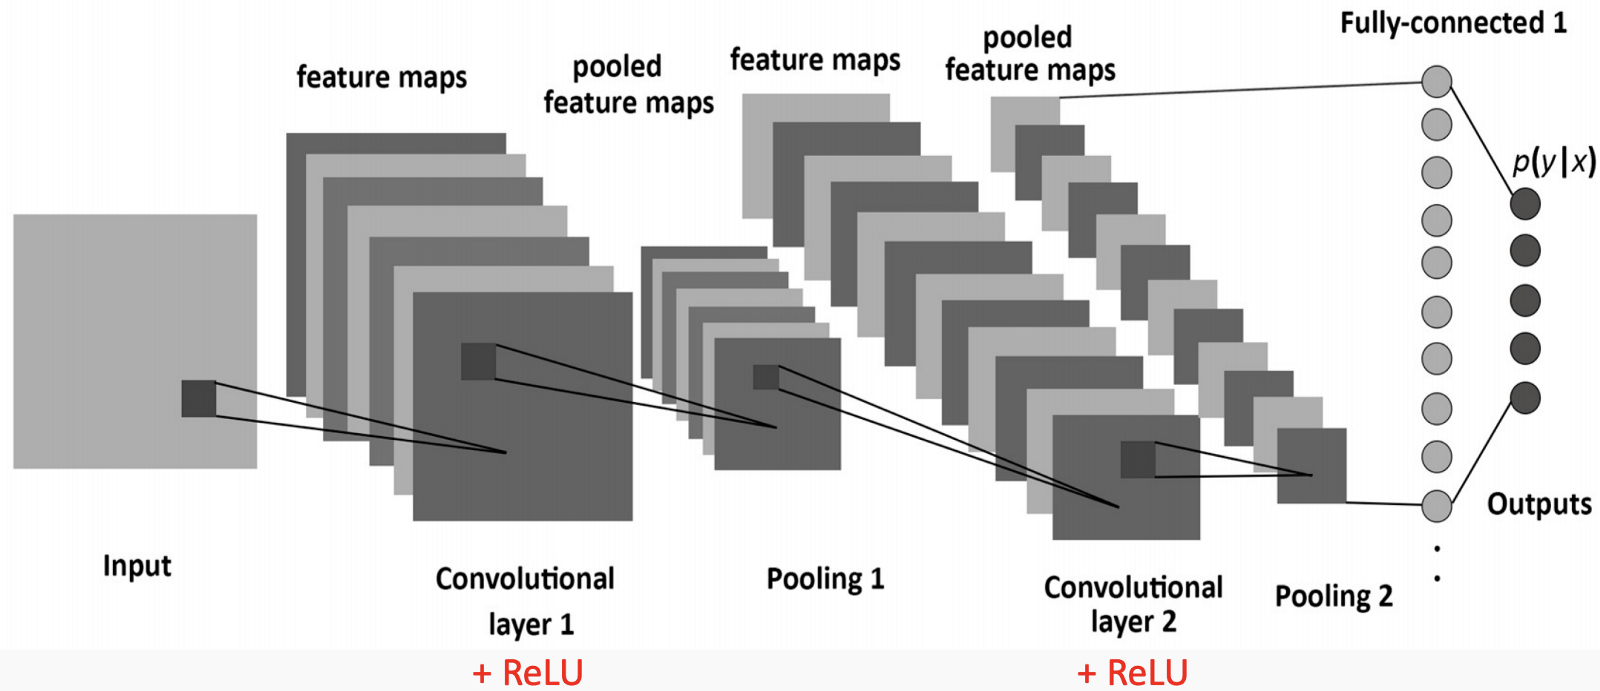
\includegraphics[width=\textwidth/4]{ETH-DS-2020/AML/Resources/cnn.png}
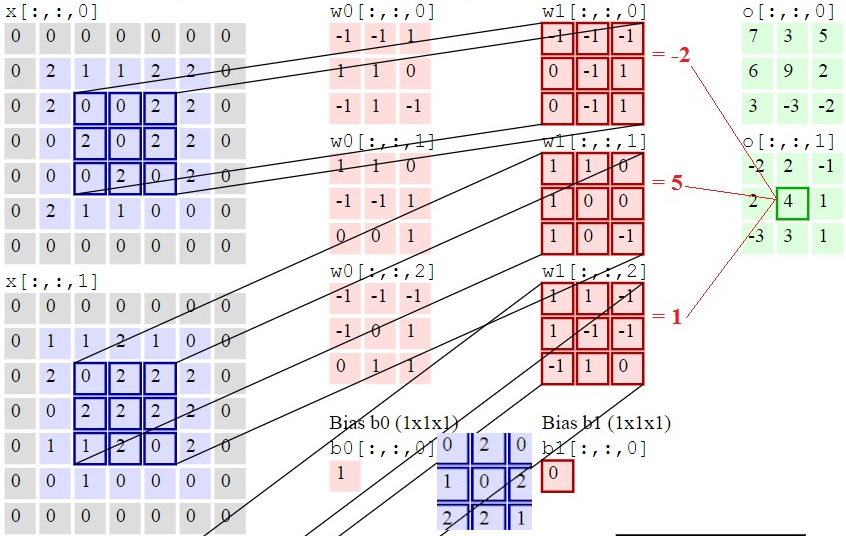
\includegraphics[width=\textwidth/4]{ETH-DS-2020/AML/Resources/conv2.jpg}
\term{Convolutional layer:} Consists of multiple stages\\
\begin{inparaitem}[$\color{mygreen} \triangleright$]
\item Conv stage: $(I*K)[i,j] = \sum_{k=-\infty}^{\infty}\sum_{l=-\infty}^{\infty}I[i-k,j-l] \cdot K[k,l]$ where $K$ is the kernel and $I$ is the 2D input(/image)\\
\item Activation: Apply some activation function\\
\item Pooling: Reduce temporal/spatial dimension (Max/Mean/Sum). To compensate for information loss, apply several kernels in convolution stage.\\
\end{inparaitem}
\term{Properties of convolutional layers:}\\
\textbf{\textcolor{mygreen}{+}} Compute efficient (backprop shares params)\\
\textbf{\textcolor{mygreen}{+}} Translation equivariant (only w.o. pooling!)\\
\textbf{\textcolor{mygreen}{+}} Parameter sharing helps reducing \#params\\
\textbf{\textcolor{red}{-}} Not all data are sequences or translationally equivariant\\
\textbf{\textcolor{red}{-}} Receptive fields are local => hard to connect distant information\\
\term{Output dim:}
$\text{dim}^{\text{out}} = \left \lfloor{\frac{\text{dim}^{\text{in}}+2P-K}{S}}\right \rfloor + 1$; $K$ kernel size, $S$ stride, $P$ padding
%\term{Application areas:}\\
%\begin{inparaitem}[$\color{mygreen} \triangleright$]
%\item Computer vision: Pyramidal structure is very common (increase number of kernels and reduce dimension in every step). Models are very deep and wide\\
%\item Natural language processing: Words first get encoded to feature vectors. Then CNN's can be applied on these vectors. Recently combinations of CNN's and attention and memory units became popular.
%\end{inparaitem}